%%%%% FORMAT %%%%%
%https://www.overleaf.com/latex/templates/template-for-submission-to-aip-publishing-journals/xhsskcchtbxf

\documentclass[%
 aip,
% jmp,
% bmf,
% sd,
% rsi,
 amsmath,amssymb,
%preprint,%
 reprint,%
%author-year,%
%author-numerical,%
% Conference Proceedings
]{revtex4-1}

\usepackage{graphicx} 
\usepackage{amsmath}
\usepackage{xcolor}
\usepackage{float}

\usepackage{graphicx}% Include figure files
\usepackage{dcolumn}% Align table columns on decimal point
\usepackage{bm}% bold math
%\usepackage[mathlines]{lineno}% Enable numbering of text and display math
%\linenumbers\relax % Commence numbering lines

\usepackage[utf8]{inputenc}
\usepackage[T1]{fontenc}
\usepackage{mathptmx}
\usepackage{etoolbox}

%% Apr 2021: AIP requests that the corresponding 
%% email to be moved after the affiliations
\makeatletter
\def\@email#1#2{%
 \endgroup
 \patchcmd{\titleblock@produce}
  {\frontmatter@RRAPformat}
  {\frontmatter@RRAPformat{\produce@RRAP{*#1\href{mailto:#2}{#2}}}\frontmatter@RRAPformat}
  {}{}
}%
\makeatother
\begin{document}

\preprint{AIP/123-QED}

\title[Markovian Innovation]{Markovian Innovation}
% Force line breaks with \\
\author{G. G. Yoshimatsu}
\author{ C. R. daCunha}%
 \email{carlo.cunha@nau.edu}
\affiliation{ 
School of Informatics, Computing, and Cyber-Systems, Northern Arizona University, Flagstaff, AZ, 86011, USA%\\This line break forced with \textbackslash\textbackslash
}%
 \homepage{https://ac.nau.edu/~cc3682}

\date{\today}% It is always \today, today,
             %  but any date may be explicitly specified

\begin{abstract}
An article usually includes an abstract, a concise summary of the work
covered at length in the main body of the article. It is used for
secondary publications and for information retrieval purposes. 
\end{abstract}

\maketitle

\section{Introduction}
Innovation dynamics are all the processes that induce change to a certain environment. The context of such environment can range from biological, such as viral mutations to scientific innovation resultant from research. Due to its abstractness, innovation can be sometimes difficult to characterize, however it can be broken down into certain main processes, such as emergence, spread and development of information throughout a system of many agents. 

\textcolor{red}{Talk about the first researchers of innovation}
\textcolor{red}{Talk about why different systems, sometimes behave in similar ways, class of universality, Markovian behavior generates such similarities?}

Statistical mechanics is a field of study that is able to break down the spread of information due to the action of many agents into simple yet very useful mathematical models and equations. In this context, we use statistical mechanics and stochastic calculus to elaborate a model that describes many innovation scenarios and allows us to extract behaviors and patterns of a system that innovates. With this we should be able to detect fraudulent data report in certain industries or the emergence of an external effect in a system, for example the effects in economical growth due to the spread of Covid-19.

One of the first researchers to study and model innovation was Frank Bass. In 1969, he proposed a simple but effective model that described the diffusion of ideas, products and technologies throughout a system or population. The model consists of a differential equation that describes the general behavior of adopters. Each adopter may be separated into innovators and imitators and each one of them will have its own innovation degree and adoption speed. Such model proved simple but useful in predicting market adoption dynamics and obsolescence.

The model proposed by Bass was built under probabilistic assumptions regarding the behaviors of individuals, something that is difficult to nail down or to avoid an over fitting of a system. In our mathematical description, we make simpler assumptions: 1. The random behavior of the system as a whole only depends on its current state, creating a Markov chain. 2. The Markov chain can be described as a diffusion process. 3. The adoption increases the number of agents adhering to a certain idea (or technology, or mutation, ...), so it must be proportional to the time. 4. The obsolescence coefficient decreases the number of individuals adhering to an idea, so it must be inversely proportional to the time. With only four simple assumptions followed by many physical systems, we are able to create a very broad model, which is most certainly not an over fitting due to its simplicity. In other words, this set of considerations is the simplest set of considerations one can make regarding a system that simultaneously explain adoption curves over time.

We also use Recurrent Neural Networks (RNNs) another statistical/stochastic tool that is very versatile in analysing time series through a feedback loop. It consists in feeding processed data back to the neural layer in order to change it in a way that it is able to predict future behaviors of a time-series. We use the RNN to better analyse the data gathered from real scenarios and compare it with what the analytical solution for the innovation model describes.

In the following chapter we introduce the model and its analytical solutions, which lead to the average number of agents adhering to a certain idea or information. This chapter is followed by a comparison via fitting between the mathematical model and data gathered from real scenarios, such as viral mutations exhibited by the Covid-19 virus, scientific articles year-over-year citations and the monthly searches of social media in the platform Google-Trends. Afterwards, we enhance the analysis by comparing the model and the data with RNNs and finally, we discuss applications of our mathematical model in predicting growth and abandonment of ideas, platforms, industries, etc. Which leads up to the conclusions and future perspectives in the area.


\section{The Model}
The state corresponding to a population of $n$ agents adhering to the new technology is described by the stochastic process $X_n$. The attachment rate per single cell for the new technology is given by $\lambda_n(t)$, whereas the detachment rate is given by $\mu_n(t)$. Moreover, the chance an individual attaches to or detaches from a technology must depend on the number of people already attached to it due to social conformity \cite{herd,EuEcon}. Therefore, we choose $\lambda_n(t)=n\lambda_0(t)$ and $\mu(t)=n\mu_0(t).$

We assume that the process $X_n$ is independent on its history, and is, consequently, Markovian. Therefore $P(X_{n+1}=x_{n+1}|X_1=x_1,X_2=x_2,\hdots,X_n=x_n)=P(X_{n+1}=x_{n+1}|X_n=x_n)$. The process $X_n$ induces a Markov chain described by:

\begin{eqnarray}
    X_n(t+\Delta_t)=&&(1-\lambda_n\Delta-\mu_n\Delta_t)X_n(t)+\lambda_{n-1}(t)\Delta_t X_{n-1}(t)\nonumber\\
    &&+\mu_{n+1}(t)\Delta_t X_{n+1}(t),
\end{eqnarray}
where $\Delta_t$ is a short period. At the limit where $\Delta_t\rightarrow 0$, the previous equation becomes:

\begin{eqnarray}
    \frac{dX_n(t)}{dt}=&&-(\lambda_n(t)+\mu_n(t))X_n(t)+\mu_{n+1}(t)X_{n+1}(t)\nonumber\\
    &&+\lambda_{n-1}(t)X_{n-1}(t).
\end{eqnarray}
The expected number of people attached to the technology at some instant $t$ and its time variation are given by:

\begin{eqnarray}
        M(t)=&&\sum_{n=1}^\infty nX_n(t)\nonumber\\
        \frac{dM(t)}{dt}&&=-\left(\lambda_0(t)+\mu_0(t)\right)\sum_{n=1}^\infty n^2X_n(t)\nonumber\\
        &&+\mu_0(t)\sum_{n=1}^\infty n(n+1)X_{n+1}(t)+\nonumber\\
        &&+\lambda_0(t)\sum_{n=1}^\infty n(n-1)X_{n-1}(t)\nonumber\\
        &&=\left(\lambda_0(t)-\mu_0(t)\right)M(t).\\
\end{eqnarray}

To account for the temporal dynamics of opinions, we propose that the attachment rate may reduce over time, and the detachment rate follows the opposite trend. This can be due to a number of factors, including the development of other technologies, temporal preferences, and the saturation of the novelty factor. \textcolor{red}{[insert references]}. Therefore, we write:

\begin{equation}
    \begin{aligned}
        \lambda_0(t)&=\frac{\alpha}{t}\\
        \mu_0(t)&=\frac{t}{\sigma^2},\\
    \end{aligned}
\end{equation}
where $\alpha$ is a growth exponent, and $\sigma$ is a characteristic time scale related to detachment. 

The time variation of the expected number of people attached to the technology becomes:

\begin{equation}
    \frac{dM(t)}{dt} = \left(\frac{\alpha}{t}-\frac{t}{\sigma^2}\right)M(t).
\end{equation}
The solution of this equation is:

\begin{equation}
    M(t)=M_0t^\alpha e^{-t^2/2\sigma^2}.
    \label{eq:number_of_attachments_over_time}
\end{equation}

Parameters $M_0$, $\alpha$ and $\sigma$ can be found using a standard Levenberg-Marquardt fitting for any specific technology. These parameters allows us to compare how different technologies grow and decay with time.

In the following section, we compare the Markovian Innovation model with existing data to obtain each of the previously mentioned parameters in real life scenarios.



\section{Results: Innovation Characterized from Data and Model} 
The first scenario concerns the yearly citations of articles published in 1980 until 2023, where we fit equation (\ref{eq:number_of_attachments_over_time}) to the the yearly citation histogram.

%==================================
% FIGURE
%==================================
\begin{figure}[H]
    \centering\includegraphics[scale=0.35, angle=270]{figs/citations.eps}
    \caption{}
    \label{fig:citations_fit}
\end{figure}

\begin{table}[H]
\begin{tabular}{|c c c c c|}
\hline
\# of Citations & RMS of Residuals & $\sigma$ & $\alpha$ & $M_{0}$    \\ \hline
1666 & 8.7546 & 15.85745 & 0.314334 & 27.8297 \\ \hline
550 & 4.03577 & 17.05420 & 0.316177 & 8.54389 \\ \hline
124 & 1.31794 & 10.50930 & 3.86016 & 5.11926e-05\\ \hline
\end{tabular}
\end{table}

If figure \ref{fig:citations_fit} there are two kinds of citation patterns, one where the number of citations increases rapidly followed by a slow decrease as time goes by. And the second kind, where the number of citations increases slowly but takes on afterwards, followed again by decrease after its peak. Both kinds of adoptions curves are well adjusted by our innovation model

The next set of data corresponds to the mutations for SARS-CoV-2 over time, where we consider the first detect strain as being the one found in Wuhan (hCoV-19/Wuhan/Hu-1/2019). The data was obtained by digitizing Fig. 4 (b) from \cite{Lee2022}, where a similar analysis is applied.
We use the mutations from root (the first found strain) as a measure of time and \textcolor{red}{tenho que ler melhor sobre o tratamento de dados que o Lee faz para obter esse gráfico...}

%==================================
% FIGURE
%==================================
\begin{figure}[H]
    \centering\includegraphics[scale=0.35, angle=270]{figs/cladecount.eps}
    \caption{}
    \label{fig:}
\end{figure}

\begin{table}[H]
\begin{tabular}{|c c c c c|}
\hline
Region & RMS of Residuals & $\sigma$ & $\alpha$ & $M_{0}$ \\ \hline
North America & 0.228755  & 2.745150 & 2.805370  & 0.126760 \\ \hline
Europe        & 0.34383 & 3.385185 & 1.393420  & 1.189050 \\ \hline
\end{tabular}
\end{table}

The third set of data correspond to Google searches of the social platforms known as Facebook and Snapchat, such data is provided openly by the Google Trends platform. We use the searches as a form of diagnosing the popularity of these two social medias that have existed for more than 10 years, the months axis represent the number of months elapsed since the first citation of the terms "Facebook" and "Snapchat" in Google Trends platform.

%==================================
% FIGURE
%==================================
\begin{figure}[H]
    \centering\includegraphics[scale=0.35, angle=270]{figs/google_trends.eps}
    \caption{}
    \label{fig:social_media}
\end{figure}

\begin{table}[H]
\begin{tabular}{|c c c c c|}
\hline
Social Media & RMS of Residuals & $\sigma$ & $\alpha$ & $M_{0}$ \\ \hline
Facebook & 8.55684  & 32.3251 & 5.4501  & 1.23955e-08 \\ \hline
Snapchat & 10.0758 & 20.1910 & 4.8127  & 2.11764e-06 \\ \hline
\end{tabular}
\end{table}

Equation \ref{eq:number_of_attachments_over_time}, agrees for most part of the data, where the adoption of both social medias assumes a power-law and the detachment is Gaussian-like. For Snapchat, approximately at month 100 since the first Google search, the rate of detachment changes, our belief is that this is caused by an external factor, such as the pandemics, as month 100 corresponds approximately to November 2019, where Covid-19 began spreading throughout the world and the countries began restricting the transit of people. The restriction most likely changed the amount of time that people interacted with social media, which may be the leading factor for changing the search dynamics for the term "Snapchat". We believe the same happened for "Facebook", whose detachment starts to deviate from the fitted function approximately at month 180 which coincides with the latter half of 2019.

\section{Relationship with Other Models}
An automaton can be described by a tuple $A=(Z,S,N,f)$ where $Z$ is a $d\times d$ lattice composed of discrete cells that can hold states $S=\{1,2,3\}$. The transition from one cell value to another 
is given by the transition function $f:S\rightarrow S$. The transition of states for a single cell takes other cells in a neighborhood into consideration. Here we used
the von Neumann neighborhood, described by the set $N(\mathbf{n}_0)=\{\mathbf{n}_k:\sum_i^d|(\mathbf{n}_k)_i-(\mathbf{n}_0)_i\leq 1\}$. The configuration of the automaton
is described by a function $c:Z\rightarrow S$ that assigns a state to each cell. The next state of a cell is given by $c(\mathbf{n}_0)^{t+1}=f(\{\mathbf{n}_m|\mathbf{n}_m\in N(\mathbf{n}_0)\}$.
The next state for a cell is determined through a random selection from the values of its neighboring cells, with the selection probabilities being proportional to the frequencies of those values. 
Therefore, each agent tends to align its state to the state of the majority of its neighbors. To avoid boundary effect, we used periodic boundary conditions.

In our simulations, the grid is randomly initiated with $S_0=\{1,2\}$. The automaton runs for $100$ steps to reach thermalization and the a new state is introduced to $n$ elements of the grid to create $S=S_0\cup\{3\}$.

Introducing the new values to the network can have different effects if the $n$ sites are dispersed or localized. 

\section{Discussions and Conclusions}
\input{tex/section_5}

\bibliographystyle{unsrt}
\bibliography{innovation}

\end{document}
